\documentclass[a4paper, twoside, 10pt, spanish]{article}


\usepackage{booktabs}
\usepackage[margin=.95in]{geometry}
\usepackage{array}
\usepackage{pdflscape}
\usepackage{multirow}
\usepackage{cite}
\usepackage{siunitx}



% Definición del tamaño de página y los márgenes:
% Si preferís menos márgenes, descomentá la línea siguiente
%\usepackage[a4paper,headheight=16pt,scale={0.7,0.8},hoffset=0.5cm]{geometry}
\usepackage[demo]{graphicx}
\usepackage{caption}
\usepackage{subcaption}
\usepackage[utf8x]{inputenc}
\usepackage[spanish]{babel}  
\usepackage[per-mode=fraction]{siunitx}
\sisetup
{
	output-decimal-marker = {.},
	exponent-product = \cdot,
        group-digits = integer,
	group-separator = {,}
}

%
% El paquete amsmath agrega algunas funcionalidades extra a las fórmulas.
% Además defino la numeración de las tablas y figuras al estilo "Figura 2.3",
% en lugar de "Figura 7". (Por lo tanto, aunque no uses fórmulas, si querés
% este tipo de numeración dejá el paquete amsmath descomentado).
%
\usepackage{amsmath, amsfonts, amssymb}
\usepackage{yhmath}
%\numberwithin{equation}{section}
%\numberwithin{figure}{section}
\numberwithin{table}{section}
% ENCABEZADO y PIE DE PÁGINA

\usepackage{fancyhdr}   % Para poder personalizarlo
\usepackage{lastpage}   % Para poder saber cuántas páginas tiene el documento
\pagestyle{fancy}
\renewcommand{\sectionmark}[1]{\markboth{}{\thesection\ \ #1}}
\fancyhead{}	% Elimino el contenido del encabezado
% Muestra la sección a la derecha (izquierda) en páginas impares (pares)
\fancyhead[RO,LE]{\rightmark}
% El siguiente texto a la derecha (izquierda) en páginas pares (impares)

\fancyfoot{}	% Elimino el contenido del pie de página
% A la izquierda (derecha) en páginas pares (impares): nro. de página / total
\fancyfoot[LE,RO]{\thepage/\pageref{LastPage}}
% Hipervínculos (enlaces) en el documento (y modificación de atributos)
\usepackage{url}
\urlstyle{tt}
\usepackage[colorlinks=true,linkcolor=black, urlcolor=blue]{hyperref}
\hypersetup{
    breaklinks,
    baseurl       = http://,
    pdfborder     = 0 0 0,
    pdfpagemode   = UseNone,
    pdfstartpage  = 1,
    pdfcreator    = {Plantilla de informe de TP para \LaTeX{}},
    bookmarksopen = true,
    bookmarksdepth= 2,% to show sections and subsections
    pdfauthor     = {Apellido~1, Apellido~2, Apellido~3},
    pdftitle      = {-},
    pdfsubject    = {Informe},
    pdfkeywords   = {}%
    }

% ==== Paquetes para TikZ ====
\usepackage{tikz}
\usetikzlibrary{arrows.meta, positioning, shapes, calc}



\usepackage{enumerate}
\usepackage{booktabs}
\usepackage{multirow}
\usepackage{pgfplots}
\pgfplotsset{compat=1.18}
\usepackage{graphicx}
\pdfcompresslevel=9

% Todas las imágenes están en el directorio imgs:
\newcommand{\imgdir}{img}
\graphicspath{{\imgdir/}}
% El paquete recomendado actualmente es minted.
% Documentación: https://www.ctan.org/pkg/minted
\usepackage[
        section,    % Numera el código según la sección
    ]{minted}
% minted provee los comandos:

% 1)  \mint[<opciones>]{<lenguaje>}<delimitador><código><delimitador>
% 2)  \mintinline[<opciones>]{<lenguaje>}<delimitador><código><delimitador>
% 3)  \inputminted[<opciones>]{<lenguaje>}{<archivo>}
\setminted[c]{
%        style=,
        linenos,            % Mostrar los números de línea
        numberfirstline,    % Numerar SIEMPRE la primera línea mostrada
        tabsize=4,          % Reemplazar las tabulaciones por 4 espacios
        autogobble          % Eliminar espacio sobrante al comienzo
    }
%%%%%%%%%%%%%%%%%%%%%%%%%%%%%%%%%%%%%%%%%%%%%%%%%%%%%%%%%%%%%%%%%%%%%%%%%%%%%
% COMANDOS UTILES
%%%%%%%%%%%%%%%%%%%%%%%%%%%%%%%%%%%%%%%%%%%%%%%%%%%%%%%%%%%%%%%%%%%%%%%%%%%%%
% los siguientes comandos permiten escribir de manera uniforme en todo el
% documento

% Para poder manejar los espacios al final de los comandos propios
\usepackage{xspace}

\usepackage{algorithm}
\usepackage{algpseudocode}

% Abreviatura de 'número' utilizando letras voladas (correcto español)
\newcommand{\Nro}{N.\textsuperscript{o}\xspace}
\newcommand{\nro}{n.\textsuperscript{o}\xspace}
%%%%%%%%%%%%%%%%%%%%%%%%%%%%%%%%%%%%%%%%%%%%%%%%%%%%%%%%%%%%%%%%%%%%%%%%%%%%%
% PAQUETES EXTRAS
%%%%%%%%%%%%%%%%%%%%%%%%%%%%%%%%%%%%%%%%%%%%%%%%%%%%%%%%%%%%%%%%%%%%%%%%%%%%%
\usepackage{circuitikz}
\usepackage{listings}
\usepackage{xcolor}

% --- Configuración para mostrar código Python ---
\lstdefinestyle{pythonstyle}{
    language=Python,
    basicstyle=\ttfamily\small,
    backgroundcolor=\color{gray!5},
    frame=single,
    framerule=0.3pt,
    rulecolor=\color{gray!50},
    keywordstyle=\color{blue!70!black},
    stringstyle=\color{orange!70!black},
    commentstyle=\color{gray!70!black}\itshape,
    showstringspaces=false,
    breaklines=true,
    tabsize=4,
    captionpos=b,
}

\lstset{style=pythonstyle}

%%%%%%%%%%%%%%%%%%%%%%%%%%%%%%%%%%%%%%%%%%%%%%%%%%%%%%%%%%%%%%%%%%%%%%%%%%%%%
% COMANDOS UTILES
%%%%%%%%%%%%%%%%%%%%%%%%%%%%%%%%%%%%%%%%%%%%%%%%%%%%%%%%%%%%%%%%%%%%%%%%%%%%%
% los siguientes comandos permiten escribir de manera uniforme en todo el
% documento

% Para poder manejar los espacios al final de los comandos propios
\usepackage{xspace}

\usepackage{algorithm}
\usepackage{algpseudocode}

%%%%%%%%%%%%%%%%%%%%%%%%%%%%%%%%%%%%%%%%%%%%%%%%%%%%%%%%%%%%%%%%%%%%%%%%%%%%%
% PAQUETES EXTRAS
%%%%%%%%%%%%%%%%%%%%%%%%%%%%%%%%%%%%%%%%%%%%%%%%%%%%%%%%%%%%%%%%%%%%%%%%%%%%%
\usepackage{float}
\usepackage{multicol}
\usepackage{gensymb}


% NO cargues otra vez \usepackage{biblatex}
% NO uses 2 \addbibresource distintos salvo que realmente quieras 2 bases
\usepackage[backend=biber,
style=numeric-comp,
sorting=none,
language=spanish,
doi=false,
isbn=false,
url=true,
eprint=false
]{biblatex}

\addbibresource{referencias.bib}
\usepackage{enumitem}

% INICIO DEL DOCUMENTO

\begin{document}

\begin{titlepage}
\centering


\includegraphics[width=0.2\textwidth]{imagenes/fiuba.pdf}\par\vspace{1cm}

{\scshape\LARGE Universidad de Buenos Aires \par}
\vspace{0.2cm}
{\scshape\Large Facultad de Ingeniería \par}
\vspace{0.2cm}
{\large 2° cuatrimestre 2026 \par}

\vspace{2cm}

{\Large \textbf{Taller de Automatización y Control}\par}

\vspace{1cm}

{\large \textbf{Trabajo Práctico N°1: Introducción al control digital}\par}

\vspace{2cm}

% Tabla de integrantes
\renewcommand{\arraystretch}{1.3}
\begin{tabular}{|m{6cm}|m{2cm}|m{5cm}|}
\hline
\multicolumn{3}{|c|}{\textbf{Integrantes Grupo N° 1}} \\
\hline
\textbf{Nombre y apellido} & \textbf{Padrón} & \textbf{Correo} \\
\hline
Francisco Javier Moya & 109899 & fjmoya@fi.uba.ar \\
\hline
Lucas Fabrizio Arias Montes & 110876 & lfarias@fi.uba.ar \\
\hline
\end{tabular}

\vfill

\end{titlepage}

\setcounter{page}{1}
\tableofcontents
\newpage


\section{Introducción}

El objetivo principal a desarrollar a lo largo de la materia será poder controlar un sistema de tipo \textit{Ball and Beam} como el que se observa en la figura \ref{fig:planta_bab}.

\begin{figure}[H]
    \centering
    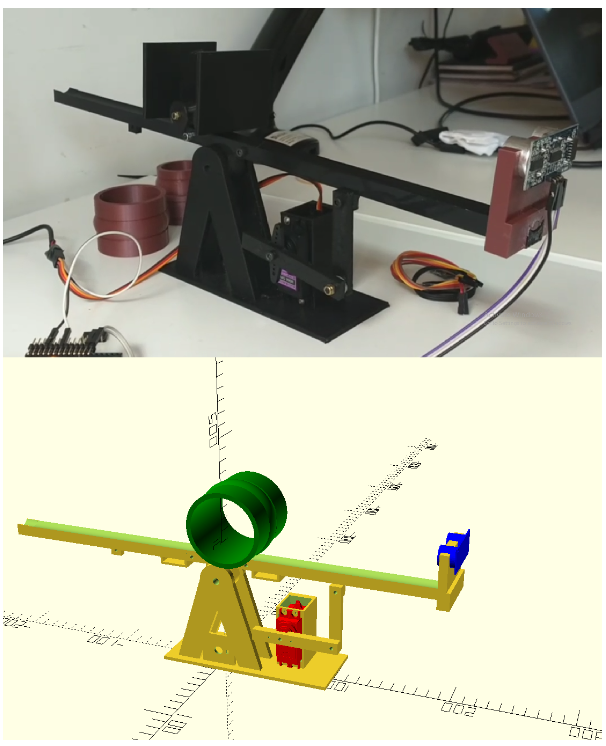
\includegraphics[width=0.5\linewidth]{imagenes/planta_BaB.png}
    \caption{Sistema Ball and Beam a controlar}
    \label{fig:planta_bab}
\end{figure}

El sistema consta de un brazo mecánico impreso en 3D sobre el cual en lugar de una bola se encuentra montado un carrito que puede rodar libremente con rozamiento despreciable. Sobre el brazo están montados un sensor de distancia ultrasónico y una IMU \textbf{MPU6050}. La inclinación del brazo es controlada por un servomotor el cual permite que el carrito se mueva a lo largo del mismo gracias a la acción de la gravedad. Así mismo, es posible además comandar un ángulo de inclinación arbitrario al brazo a través de un potenciómetro, convirtiendo la tensión medida por el mismo en un ángulo mediante un software que se ejecuta en un microcontrolador Arduino Nano, a donde también se conecta toda la electrónica del sistema.\\

En este trabajo práctico se buscarán analizar las limitaciones que presentan los sensores y actuadores que serán utilizados para controlar el sistema así como las limitaciones adicionales que existen a la hora de enviar datos a través del puerto serie de Arduino, en particular para variables de tipo \texttt{float}. Todo ello con el fin de conocer las limitaciones que presenta el hardware con el que se va a trabajar a lo largo de la cursada y utilizar toda la información recopilada en etapas de diseño posteriores.

\subsection{Componentes utilizados}

\textcolor{red}{Falta arreglar el tema de las referencias que no lo pude arreglar todavía.}

Para la implementación del sistema \textit{Ball and Beam} se utilizó un
Arduino Nano como unidad de procesamiento y control. La posición del móvil
sobre la barra se mide mediante un sensor ultrasónico HC-SR04, mientras que
la inclinación de la barra se estima utilizando una unidad de medición
inercial MPU6050. Como actuador se emplea un servomotor MG996R Digital High
Torque, encargado de modificar la inclinación de la barra. Finalmente, un
potenciómetro permite establecer manualmente la referencia de posición del
sistema.

A continuación se presentan los principales componentes utilizados y la
función que cumple cada uno dentro del sistema.

\subsubsection{Sensor ultrasónico HC-SR04}

Para medir la posición del móvil sobre la barra se utiliza el sensor
ultrasónico HC-SR04 (fig. \ref{fig:hc_sr04}). Este dispositivo determina la distancia a un objeto
a partir del tiempo de vuelo de una señal ultrasónica: el sensor emite un
pulso y mide el tiempo transcurrido hasta la recepción del eco producido
por el objeto \cite{hcsr04}.

El módulo posee cuatro terminales: alimentación (\texttt{VCC}), tierra
(\texttt{GND}), disparo (\texttt{TRIG}) y recepción del eco
(\texttt{ECHO}). El Arduino inicia cada medición mediante el terminal
\texttt{TRIG} y determina la distancia a partir de la duración del pulso
obtenido en \texttt{ECHO}.

\begin{figure}[H]
    \centering
    % Reemplazar por la imagen correspondiente
    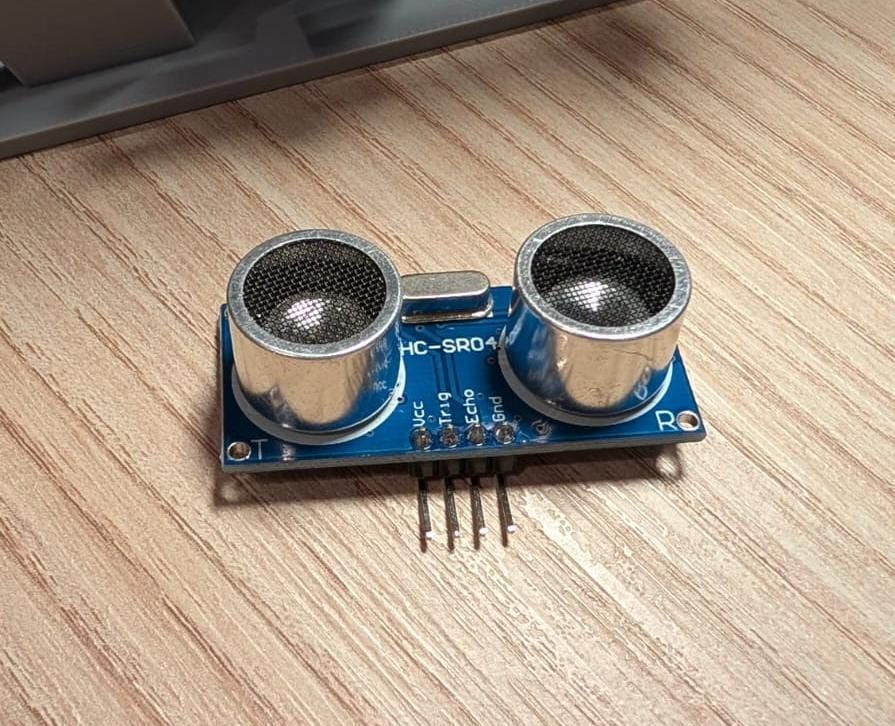
\includegraphics[width=0.45\textwidth]{imagenes/hc_sr04.jpeg}
    \caption{Sensor ultrasónico HC-SR04 utilizado para medir la posición
    del móvil sobre la barra.}
    \label{fig:hc_sr04}
\end{figure}


\subsubsection{Unidad de medición inercial MPU6050}

Para estimar la inclinación de la barra se utiliza una unidad de medición
inercial (IMU) basada en el MPU6050 (fig. \ref{fig:mpu6050}). Este dispositivo integra un
acelerómetro de tres ejes y un giróscopo de tres ejes \cite{MPU6050}.

En esta aplicación, las mediciones del acelerómetro y del giróscopo se
utilizan para obtener una estimación del ángulo de inclinación de la barra.
La combinación de ambas mediciones permite aprovechar la información
proporcionada por los dos sensores y obtener una estimación adecuada del
ángulo durante el funcionamiento del sistema.

La comunicación entre el MPU6050 y el Arduino Nano se realiza mediante el
protocolo I$^2$C.

\begin{figure}[H]
    \centering
    % Reemplazar por la imagen correspondiente.
    % Conviene que en la fotografía se pueda identificar la orientación
    % de los ejes x, y, z de la IMU.
    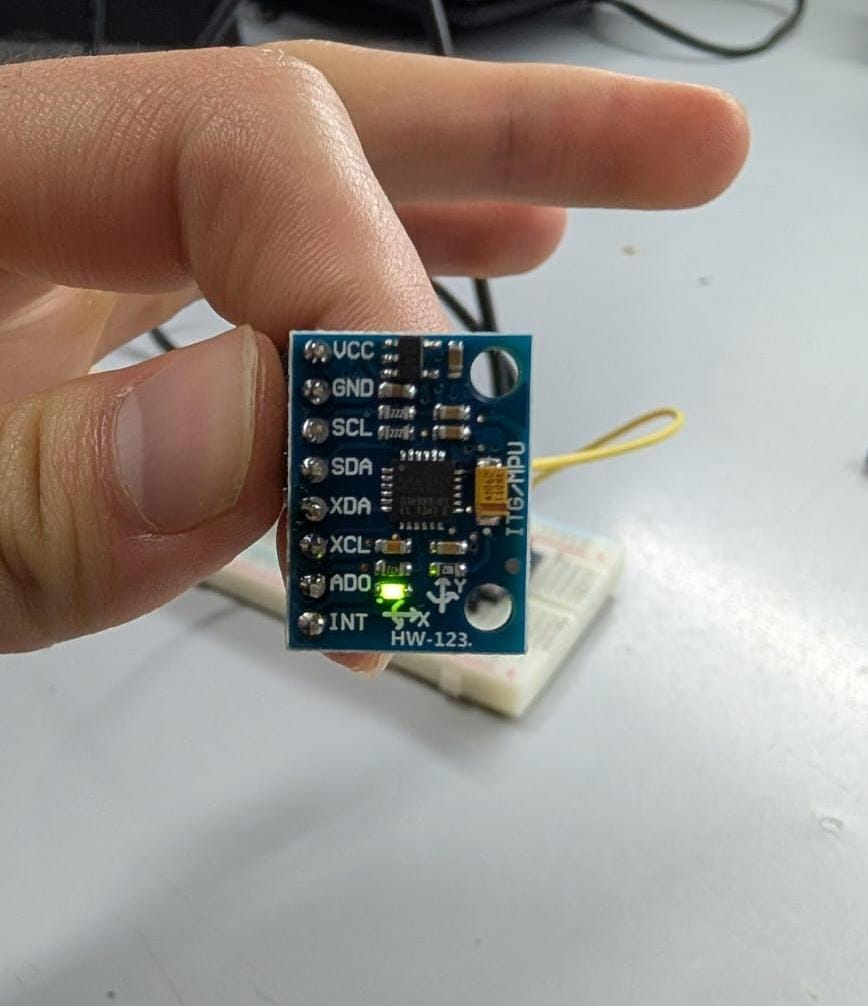
\includegraphics[width=0.45\textwidth]{imagenes/mpu6050.jpeg}
    \caption{Unidad de medición inercial MPU6050 utilizada para estimar
    el ángulo de inclinación de la barra.}
    \label{fig:mpu6050}
\end{figure}


\subsubsection{Servomotor MG996R}

La inclinación de la barra se modifica mediante un servomotor MG996R
\textit{Digital High Torque}, que constituye el actuador del sistema (fig. \ref{fig:mg996r}). El Arduino
genera la señal de comando correspondiente al ángulo deseado del servo,
produciendo de esta manera el movimiento mecánico necesario para modificar
la inclinación de la barra.

El análisis de la resolución angular, la señal de comando y el tiempo de
respuesta del servomotor se desarrolla posteriormente en la sección
correspondiente a las limitaciones de los actuadores.

\begin{figure}[H]
    \centering
    % Reemplazar por la imagen correspondiente
    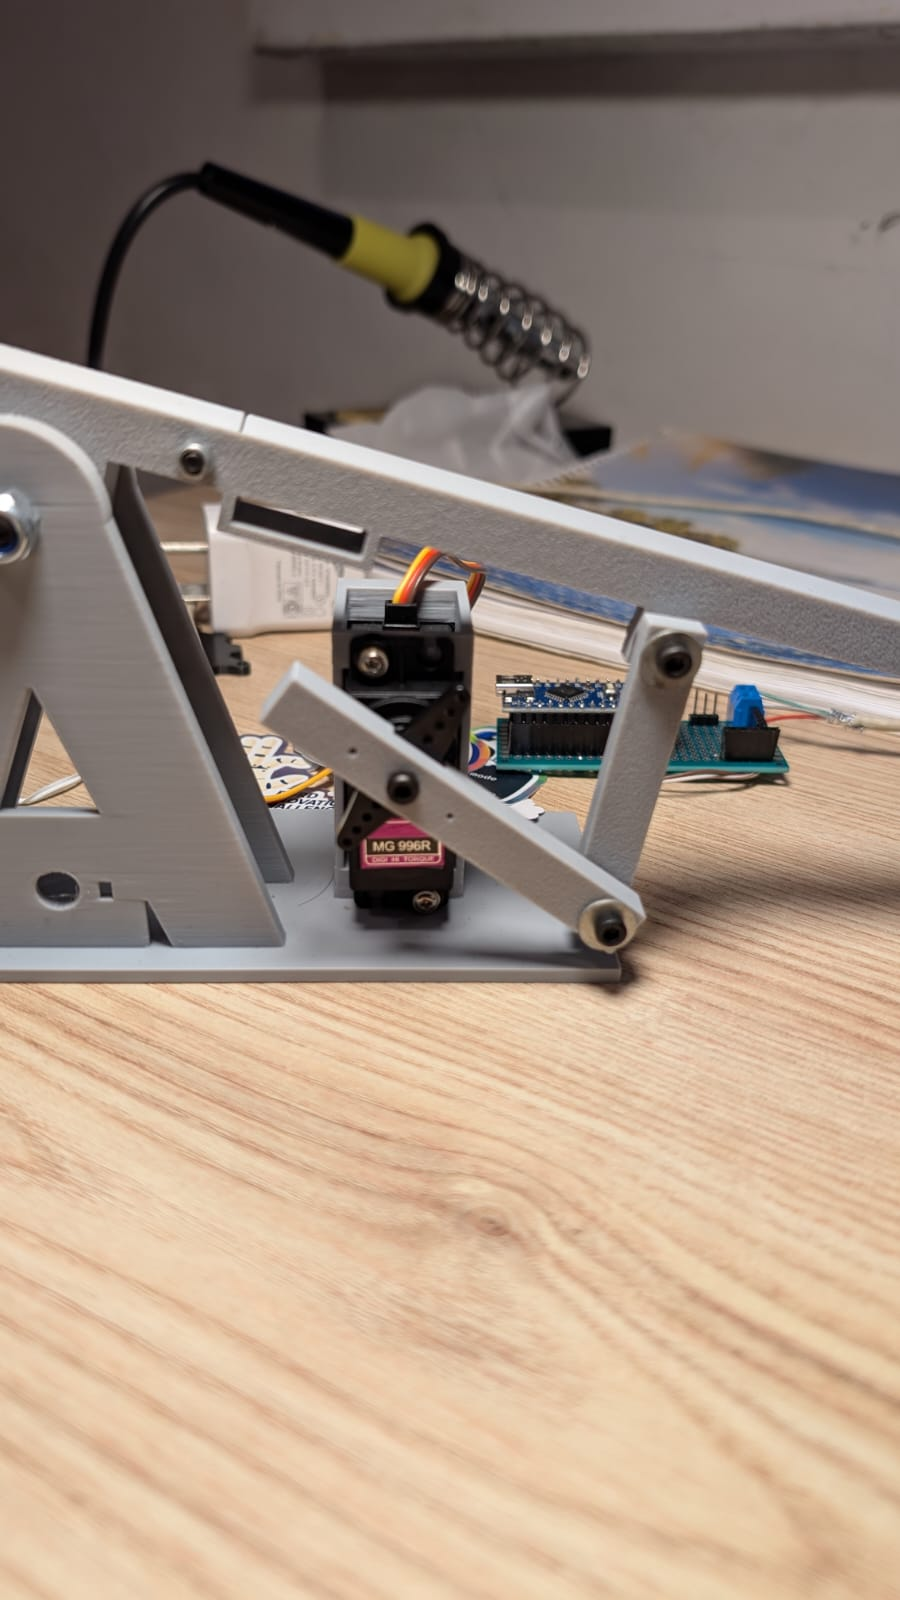
\includegraphics[width=0.45\textwidth]{imagenes/mg996r.jpeg}
    \caption{Servomotor MG996R utilizado como actuador del sistema.}
    \label{fig:mg996r}
\end{figure}


\subsubsection{Arduino Nano}

El procesamiento de las mediciones y la generación de las señales de
control se realizan mediante un Arduino Nano (fig. \ref{fig:arduino_nano}). El microcontrolador se
encarga de adquirir las señales provenientes de los distintos sensores,
procesarlas y generar la señal de comando para el servomotor.

Además, permite la comunicación con una computadora mediante el puerto
serie, utilizada durante las pruebas y la adquisición de datos del sistema.

\begin{figure}[H]
    \centering
    % Reemplazar por la imagen correspondiente
    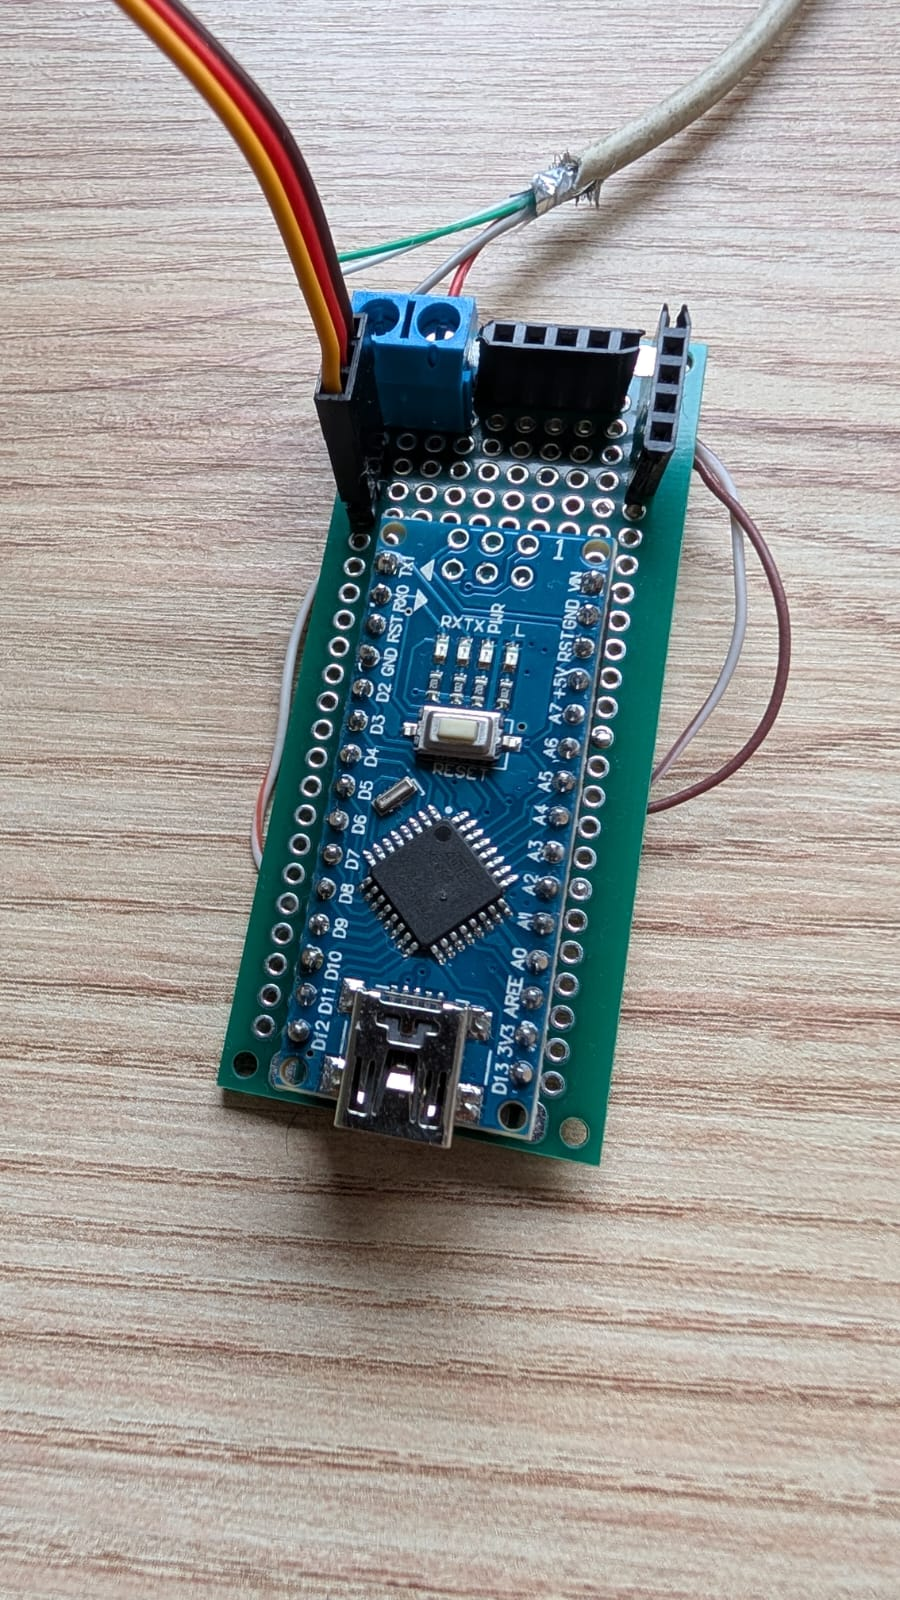
\includegraphics[width=0.45\textwidth]{imagenes/arduino_nano.jpeg}
    \caption{Arduino Nano utilizado para la adquisición, procesamiento
    y control del sistema.}
    \label{fig:arduino_nano}
\end{figure}


\subsubsection{Potenciómetro}

El sistema cuenta además con un potenciómetro utilizado para establecer
manualmente la referencia de posición del móvil (fig. \ref{fig:potenciometro}). La tensión presente en
su terminal central depende de la posición angular del mismo y es adquirida
por una entrada analógica del Arduino Nano.

A partir de esta medición, el valor obtenido por el conversor
analógico-digital del microcontrolador se transforma en una referencia de
posición válida para el sistema.

\begin{figure}[H]
    \centering
    % Reemplazar por una fotografía del potenciómetro utilizado
    \includegraphics[width=0.45\textwidth]{potenciometro}
    \caption{Potenciómetro utilizado para establecer la referencia de
    posición del sistema.}
    \label{fig:potenciometro}
\end{figure}

\section{Limitaciones de los sensores}

\subsection{Potenciómetro}

Para analizar la máxima resolución en la lectura del potenciómetro lo primero a considerar es que el conversor analógico digital (ADC) del Arduino Nano posee una resolución de 10 bits. Esto significa que el arduino posee $2^{10} = 1024$ valores distintos para representar la tensión medida en el potenciómetro, con lo cual dicha tensión será mapeada a un número entero entre $0$ y $1023$. Dado que el potenciómetro se alimenta de los $5$ V de referencia que provee el Arduino, la tensión de entrada estará entre $0$ y $5$ V, y por ende la máxima resolución en tensión alcanzable se puede calcular como:

\begin{equation}
    \Delta V = \frac{5 \ \text{V}}{1024} \approx 4,88 \ \text{mV} 
\end{equation}

Para obtener un valor de ángulo en grados a partir del potenciómetro, se debe mapear de alguna manera la lectura obtenida del ADC a través de alguna función que relacione dicha lectura con un ángulo. Considerando que los ángulos a comandar al brazo estarán en el rango $\theta \in [0 \degree, 180 \degree]$, y que el potenciómetro a utilizar es de tipo lineal, se puede utilizar la siguiente relación lineal para mapear las lecturas del ADC:

\begin{equation}
    \theta = \frac{\theta_{max} - \theta_{min}}{x_{max} - x_{min}} \ x = \frac{180 \degree}{1023} \ x
\end{equation}

Donde $x$ representa la lectura obtenida del ADC, con $x \in [0, 1023]$.

Por ende se deduce que la resolución angular será:

\begin{equation*}
    \Delta \theta = \frac{180 \degree}{1024} \approx 0,176 \degree
\end{equation*}

En cuanto al tiempo de medición requerido, aquí entran en juego varios factores. En primer lugar se debe considerar el tiempo que necesita el ADC del Arduino para transformar el valor leído del potenciómetro a un número entre $0$ y $1023$. Luego hay que considerar que además ese valor debe ser multiplicado por una constante que está guardada en una variable de tipo \texttt{float}, lo cual agrega un tiempo de procesamiento extra debido a que se debe manejar aritmética de punto flotante. Teniendo en cuenta estos factores, se estimó experimentalmente el tiempo de medición utilizando el código que figura en la sección \ref{sec:codigo_pote} del apéndice, donde la medición arrojó un valor mínimo de $108 \ \mu$s y un máximo de $116 \ \mu$s, con lo cual:

\begin{equation*}
    \hat{t}_{med} \approx (112 \pm 4) \ \mu s
\end{equation*}

\subsection{Sensor de distancia ultrasónico}

A partir de la hoja de datos del sensor, se obtuvo que la máxima resolución en distancia es de $\Delta x = 0,3$ cm. Considerando que la velocidad del sonido en CNPT es $v_s = 343$ m/s, la máxima resolución temporal se obtiene como:

\begin{equation*}
    \Delta t = 2 \frac{\Delta x}{v_s} \approx 17,49 \ \mu s
\end{equation*}

En cuanto al tiempo de medición, éste dependerá de la distancia a la que se encuentre el objeto, ya que la onda debe viajar hasta el carrito, rebotar en él, y volver hasta el sensor. Considerando que la barra mide $l \approx 35$ cm, se puede asegurar que el tiempo de medición será como mucho el tiempo que le tome a la onda el recorrer la barra completa ida y vuelta, por lo que:

\begin{equation*}
    t_{max} = 2 \frac{l}{v_s} \approx 2,04 \ ms
\end{equation*}

\subsection{Unidad de medición inercial (IMU MPU6050)}

En esta parte, se busca responder a la siguiente pregunta: ¿cual es el cambio de ángulo más chico que puede detectar la IMU? 

La medición depende exclusivamente del acelerómetro triaxial interno, ya que el giróscopo únicamente registra velocidad angular y presenta una deriva temporal acumulativa al integrarse. 

Para medir la inclinación de la barra se utiliza la componente de la acelración de la gravedad sobre el eje longitudinal del acelerómetro (en el caso de este proyecto es $a_y$). El MPU6050 posee un ADC de $16\text{ bits}$ en complemento a 2 para cada eje (es decir, mide tanto números positivos como negativos), y permite configurar el acelerómetro en distintos rangos de medición. Con el objetivo de buscar la máxima sensibilidad del componente, se selecciona el rango más chico: $\pm 2g \text{AFS_SEL = 0}$.

En esta configuración, la sensibilidad nominal indicada por el fabricante es de:

\begin{equation*}
    S = 16,384\ \frac{\text{LSB}}{g}
\end{equation*}

Esto significa que una variación de una unidad en la salida digital del sensor corresponde a aproximadamente:

\begin{equation*}
    \Delta a = \frac{1}{16,384}g
\end{equation*}

Por otro lado, si la barra forma un ángulo $\theta$ con la horizontal, la componente de la gravedad sobre el eje longitudinal puede expresarse como:

\begin{equation*}
    a_y = g\sin(\theta)
\end{equation*}

Para ángulos chicos, $\sin(\theta)\approx\theta$ (teniendo en cuenta que el ángulo tiene que estar expresado en radianes), por lo que:

\begin{equation*}
    $a_x\approx g\theta$
\end{equation*}

De esta manera, considerando únicamente la resolución del ADC, el camino mínimo de ángulo que podría detectarse sería de aproximadamente:

\begin{equation*}
    \Delta\theta \approx \frac{1}{16,384}\text{ rad}
    \approx 0{,}0035^\circ
\end{equation*}

Sin embargo, este valor representa solamente la resolución teórica del sistema y no la resolución real de la medición. El acelerómetro presenta un nivel de ruido propio que limita la capacidad de detectar cambios tan chicos. Para una densidad de ruido de aproximadamente $400\mu g/\sqrt{\text{Hz}}$ (densidad espectral de ruido, es una forma de decir qué tan grande es ese ruido por unidad de ancho de banda) y un ancho de banda de $\SI{44}{\hertz}$, el ruido RMS estimado es del orden de $2{,}65\text{m}g$.

Este valor es considerablemente mayor que la variación correspondiente a un solo LSB del ADC y equivale, cerca de la posición horizontal, a una variación angular del orden de:

\begin{equation*}
    \Delta\theta_{\text{ruido}}\approx 0{,}15^\circ
\end{equation*}

Por lo tanto, aunque el ADC presenta una resolución teórica de aproximadamente $0{,}0035^\circ$, la resolución angular efectiva estará principalmente limitada por el ruido del acelerómetro. Esta resolución puede mejorarse mediante promediado de las mediciones o mediante un filtrado adicional en el microcontrolador.

Por otro lado, el tiempo necesario para obtener una muestra de la IMU depende, entre otros factores, de la velocidad de comunicación del bus I$^2$C. Para calcular el tiempo mínimo de transferencia, se considera la lectura de los ejes del acelerómetro, lo que requiere obtener $6 \text{bytes}$ de datos.

Mediante una \textit{burst read}, se comienza indicando al MPU6050 la dirección del primer registro del acelerómetro, \texttt{ACCEL_XOUT_H} (\texttt{0x3B}), y luego se leen consecutivamente a los ejes $X$, $Y$ y $Z$.

La cantidad de pulsos de reloj del bus necesarios para la lectura principal puede estimarse considerando:

\begin{itemize}
    \item Dirección del dispositivo en modo escritura + ACK: $9$ ciclos.
    \item Dirección del registro inicial + ACK: $9$ ciclos.
    \item Dirección del dispositivo en modo lectura + ACK: $9$ ciclos.
    \item Lectura de 14 bytes, incluyendo los bits de ACK/NACK: $14\times9=126$ ciclos.
\end{itemize}

Por lo tanto, la lectura principal requiere:

\begin{equation*}
N_{14\text{ bytes}} = 9+9+9+126=153
\end{equation*}

Cada lectura adicional de un registro de un byte requiere $9+9+9+9=36$ pulsos. En consecuencia, para las tres transacciones realizadas por la biblioteca:

\begin{equation*}
N_{\text{total}} = 153 + 2\times36 = 225
\end{equation*}

Las condiciones de START, repeated START y STOP imponen tiempos adicionales, pero no se cuentan como un pulso de datos fijo. Para una velocidad de bus configurada de $400\,\text{kHz}$, correspondiente al modo rápido de I$^2$C utilizado en el ensayo, el período de cada ciclo es:

\begin{equation*}
T_{\text{I}^2\text{C}}=
\frac{1}{400\,000\,\text{Hz}}
=2{,}5\,\mu\text{s}
\end{equation*}

Por lo tanto, el tiempo teórico de transferencia resulta:

\begin{equation*}
t_{\text{bus}}=
N_{\text{total}}T_{\text{I}^2\text{C}}
=225\times2{,}5\,\mu\text{s}
=562{,}5\,\mu\text{s}
\end{equation*}

Este valor representa únicamente una estimación del tiempo ocupado por los pulsos de reloj de las transferencias I$^2$C. El tiempo total de medición incluye además los tiempos entre transacciones, la ejecución de la biblioteca, las conversiones de unidades y el cálculo trigonométrico del ángulo. Por este motivo, se determinará experimentalmente midiendo con \texttt{micros()} desde antes de llamar a \texttt{getEvent()} hasta obtener el ángulo en grados, sin incluir la impresión por puerto serie dentro del intervalo cronometrado.

Finalmente, debe distinguirse el tiempo de comunicación del tiempo de actualización de los datos dentro del MPU6050. La frecuencia de actualización del acelerómetro establece cada cuánto tiempo se dispone de una nueva muestra, mientras que el cálculo anterior determina cuánto tiempo demanda transferir una muestra ya disponible desde el sensor hacia el microcontrolador.

El envío posterior a MATLAB constituye otra etapa: los datos adquiridos por I$^2$C se procesan en Arduino y luego se transmiten a la computadora por el puerto serie, configurado a $115\,200$ bit/s. Los bytes transmitidos dependen de la trama del programa; por ejemplo, en la adquisición de seis componentes de la Práctica 2 se envían $4 \text{bytes}$ de cabecera (\texttt{abcd}) y seis valores \texttt{float} de $4 \text{bytes}$, es decir, $28 \text{bytes}$ por trama. Con formato 8-N-1 se transmiten 10 bits por byte, por lo que esa trama requiere nominalmente $28\times10/115\,200\approx2{,}43$ ms sobre el enlace serie. Este tiempo no forma parte de la lectura I$^2$C ni representa por sí solo la latencia hasta que MATLAB recibe y procesa los datos. Las tramas de ángulos de la Práctica 3 tienen otro tamaño, según las variables enviadas.

Para evaluar el funcionamiento en reposo se registraron 2000 mediciones durante aproximadamente 20 segundos, manteniendo fija la IMU. Se utilizó el filtro complementario con $\alpha=0{,}92$, un período de muestreo programado de $\SI{10}{\milli\second}$ ($\SI{100}{\hertz}$), rango del acelerómetro de $\pm2g$ y comunicación I$^2$C a $SI{400}{\kilo\hertz}$. Antes del registro se calibró el giróscopo mediante el promedio de 500 lecturas en reposo y se dejó funcionar el filtro durante 3 segundos para descartar el transitorio inicial.

El ángulo complementario presentó un valor medio de $-0{,}275867^\circ$, una desviación estándar de $0{,}016850^\circ$ y una variación pico a pico de $0{,}109921^\circ$. Esto indica que, aún con la barra quieta, el ángulo estimado presenta pequeñas fluctuaciones alrededor de su valor medio.

Tomando tres veces la desviación estándar como criterio de resolución práctica estimada, se obtiene:
\begin{equation*}
    \Delta\theta_{\text{práctica}} = 3\sigma \approx 0{,}050549^\circ \approx 0{,}051^\circ.
\end{equation*}
Este valor es mayor que el paso de cuantización ideal de $0{,}0035^\circ$ y caracteriza el nivel de ruido de la estimación filtrada en las condiciones del ensayo. La dispersión medida es menor que la estimación de ruido del acelerómetro presentada anteriormente, pero corresponden a señales distintas: aquí se evalúa la salida del filtro complementario. El criterio de $3\sigma$ es orientativo y no constituye una verificación de exactitud ni garantiza la detección de cambios de ese tamaño; para comprobarlo sería necesario realizar ensayos con variaciones angulares conocidas.

En el ensayo previo se obtuvo un tiempo promedio de lectura con Adafruit y cálculo del filtro complementario de $\SI{1,723}{\milli\second}$. Con valores observados entre $1{,}572$ y $\SI{1,748}{\milli\second}$. Este tiempo es mayor que la estimación del bus I$^2$C porque incluye también la ejecución del programa y el procesamiento de los datos. No incluye la calibración inicial ni el envío posterior a MATLAB.

\section{Limitaciones de los actuadores}


\subsection{Servomotor MG996R}

El actuador utilizado para modificar la inclinación de la barra es un
servomotor MG996R \textit{Digital High Torque}. Según la hoja de datos, el
servomotor puede controlarse mediante una señal de pulsos periódicos,
utilizando un ancho de pulso de aproximadamente $1\,ms$ para una posición
extrema, $1.5\,ms$ para la posición central y $2\,ms$ para la posición
opuesta \cite{mg996r}. Además, el fabricante especifica un \textit{dead
band width} de $5\,\mu s$, que representa una variación del ancho de pulso
por debajo de la cual el cambio de posición puede no ser detectado por el
servo.

Para estudiar el comportamiento del actuador en la implementación planteada,
se realizó una prueba experimental variando el ancho del pulso aplicado al
servomotor. Se encontró que el rango de funcionamiento utilizado por la
planta se encuentra aproximadamente entre $550\,\mu s$ y $1600\,\mu s$.
Para valores inferiores no se observaron variaciones adicionales apreciables en la inclinación de la barra. Mientras que para valores superiores a este límite, la barra comenzaba a inclinarse nuevamente en sentido contrario.

Tomando como referencia la posición horizontal de la barra, se obtuvo
experimentalmente que un ancho de pulso de $900\,\mu s$ corresponde a un
ángulo de aproximadamente $0^\circ$. Los valores obtenidos para los
extremos del rango utilizado fueron:

\begin{table}[H]
    \centering
    \begin{tabular}{cc}
        \toprule
        Ancho de pulso & Ángulo de la barra \\
        \midrule
        $550\,\mu s$ & $-14.8^\circ$ \\
        $900\,\mu s$ & $0^\circ$ \\
        $1600\,\mu s$ & $22.3^\circ$ \\
        \bottomrule
    \end{tabular}
    \caption{Relación experimental entre el ancho de pulso aplicado al
    servomotor y el ángulo de inclinación de la barra.}
    \label{tab:servo_pwm_angulo}
\end{table}

La estimación del ángulo se realizó utilizando la IMU MPU6050 y un filtro
complementario que combina las mediciones del acelerómetro y del
giróscopo.


La hoja de datos especifica un \textit{dead band} de $5\,\mu s$
\cite{mg996r}. Por lo tanto, aunque sea posible modificar el ancho del
pulso en pasos menores, una variación inferior a este valor puede no
producir un cambio de posición observable en el eje del servomotor.

Considerando el rango de control indicado en la hoja de datos, de
$1\,ms$ a $2\,ms$, y tomando los $180^\circ$ de recorrido aproximado
indicados por el fabricante, se obtiene como estimación de la relación
entre el ancho de pulso y el ángulo:

\begin{equation*}
\frac{\Delta\theta}{\Delta PWM}
=
\frac{180^\circ}{1000\,\mu s}
=
0.18^\circ/\mu s.
\end{equation*}

De esta manera, una variación de $5\,\mu s$, correspondiente al
\textit{dead band} especificado por el fabricante, equivale
aproximadamente a:

\begin{equation*}
\Delta\theta_{\mathrm{dead\,band}}
=
5\,\mu s \cdot 0.18^\circ/\mu s
=
0.9^\circ.
\end{equation*}

Por lo tanto, la resolución angular teórica asociada al \textit{dead band}
del servomotor es del orden de $0.9^\circ$. Este valor debe interpretarse
como una estimación, ya que la relación entre el ancho de pulso y el ángulo
real depende del servo y de la mecánica utilizada.

Además de la resolución teórica, se analizó experimentalmente cuál es la
mínima variación del ancho de pulso que produce un movimiento observable
en la barra. Se encontró que variaciones del ancho de pulso de aproximadamente $5 \ \mu s$ ya producían desplazamientos (cómo especificaba el fabricante) apreciables de la barra. Por ejemplo, partiendo de un pulso de $900 \ \mu s$, tanto un incremento hasta $905 \ \mu s$ como una disminución hasta $895 \ \mu s$ generaban una variación observable en la inclinación. Por lo tanto, para la implementación planteada se considera una variación
mínima observable de:

\begin{equation*}
\Delta PWM_{\min} \approx 5\,\mu s.
\end{equation*}

Para estimar qué variación angular representa este cambio, se pueden
considerar los dos lados del punto de equilibrio por separado. Para el
lado negativo se obtuvo:

\begin{equation*}
\frac{\Delta\theta}{\Delta PWM}
=
\frac{14.8^\circ}{900\,\mu s-550\,\mu s}
=
0.0423^\circ/\mu s.
\end{equation*}

Por lo tanto, una variación de $5\,\mu s$ representa aproximadamente:

\begin{equation*}
\Delta\theta_{\min}
\approx
5\,\mu s \cdot 0.0423^\circ/\mu s
\approx
0.21^\circ.
\end{equation*}

Para el lado positivo se obtiene:

\begin{equation*}
\frac{\Delta\theta}{\Delta PWM}
=
\frac{22.3^\circ}{1600\,\mu s-900\,\mu s}
=
0.0319^\circ/\mu s,
\end{equation*}

lo que da:

\begin{equation*}
\Delta\theta_{\min}
\approx
5\,\mu s \cdot 0.0319^\circ/\mu s
\approx
0.16^\circ.
\end{equation*}

Los resultados muestran que la relación entre el ancho de pulso y el
ángulo de la barra no es perfectamente lineal ni simétrica. Para la
implementación propuesta, una variación de $5\,\mu s$ del ancho de pulso produce
aproximadamente una variación angular observable de entre
$0.16^\circ$ y $0.21^\circ$.

\subsubsection{Mapeo entre ancho de pulso y ángulo de la barra}

Sea $p$ el ancho del pulso alto expresado en $\mu s$. A partir de los tres
puntos de la tabla \ref{tab:servo_pwm_angulo}, se propone una interpolación
lineal por tramos que conserva la posición horizontal medida:
\begin{equation}
\hat\theta_b(p)=
\begin{cases}
\displaystyle \frac{14.8}{350}(p-900)^\circ, & 550\leq p\leq900,\\[4pt]
\displaystyle \frac{22.3}{700}(p-900)^\circ, & 900<p\leq1600.
\end{cases}
\label{eq:mapa_servo}
\end{equation}
Por ejemplo, $895\,\mu s$ corresponde a $-0.211^\circ$ y
$905\,\mu s$ a $0.159^\circ$. El mapeo inverso, con $\theta_b$ expresado
en grados y $p$ en $\mu s$, es:
\begin{equation}
p(\theta_b)=
\begin{cases}
900+\displaystyle\frac{350}{14.8}\theta_b, & -14.8\leq\theta_b\leq0,\\[4pt]
900+\displaystyle\frac{700}{22.3}\theta_b, & 0<\theta_b\leq22.3.
\end{cases}
\end{equation}
Este modelo estima el ángulo de la barra, no el del eje del servo, y no
debe extrapolarse fuera del intervalo ensayado. Las pendientes son promedios
de cada tramo; para caracterizar la no linealidad y la histéresis harían falta
más puntos, medidos en ambos sentidos. El ancho de pulso determina la
consigna: no es el tiempo durante el cual se mueve el motor.

\subsubsection{Tiempo estimado y medido para un desplazamiento de $30^\circ$}

La especificación de velocidad del MG996R indica $0.17\,s/60^\circ$ a
$4.8\,V$ y $0.14\,s/60^\circ$ a $6\,V$ \cite{mg996r_velocidad}.
Suponiendo velocidad constante, el tiempo de recorrido para una variación
de $30^\circ$ en el eje del servo se estima como:
\begin{equation}
\hat t_{30}=\frac{30^\circ}{60^\circ}t_{60}=
\begin{cases}
85\,ms, & V=4.8\,V,\\
70\,ms, & V=6\,V.
\end{cases}
\end{equation}
Son estimaciones nominales, no mediciones del sistema montado ni tiempos
de establecimiento garantizados. La carga, la aceleración, el frenado y la
tensión de alimentación pueden modificar el resultado. No se conoce aquí
la tensión efectiva del ensayo, por lo que se conservan ambos casos.

La biblioteca \texttt{Servo} mantiene un intervalo de refresco nominal de
$20\,ms$ \cite{arduino_servo}. Una orden puede esperar aproximadamente
entre $0$ y $20\,ms$ hasta el siguiente pulso; sumando sólo esa espera al
recorrido nominal se obtienen $85$--$105\,ms$ a $4.8\,V$ y
$70$--$90\,ms$ a $6\,V$, sin incluir otros retardos internos.

Si los $30^\circ$ se refieren a la barra, estos tiempos no pueden aplicarse
directamente: falta la relación cinemática entre el eje y la barra. Por
ejemplo, pasar de $-10^\circ$ a $20^\circ$ en la barra corresponde, según el
mapeo, a pasar aproximadamente de $664$ a $1528\,\mu s$, pero eso no
determina el giro del eje.
Cronometrar únicamente \texttt{writeMicroseconds()} mide la actualización
de la consigna, no el movimiento mecánico.

Para medir la respuesta del sistema montado, se realizó este desplazamiento
de $-10^\circ$ a $20^\circ$ de la barra mediante el programa
\texttt{t\_respuesta\_servo.ino}, registrando el ángulo estimado con la IMU
y el filtro complementario cada $10\,ms$. Se midió el tiempo desde la orden
hasta la entrada en una banda de $\pm1^\circ$ alrededor del ángulo final,
confirmando que la medición permaneciera dentro de ella durante $100\,ms$.
En el ensayo se obtuvo:
\begin{equation*}
t_{\text{llegada, barra}} = 391{,}9\,ms \approx 0{,}39\,s.
\end{equation*}
La llegada se confirmó a los $491{,}9\,ms$, con una lectura de
$20{,}56^\circ$; los $100\,ms$ de confirmación no se suman al tiempo de
llegada informado. Este resultado corresponde a un único ensayo e incluye
la espera de aplicación del comando, la respuesta mecánica del conjunto
y los retardos de la IMU y del filtro. El muestreo de $10\,ms$ limita la
resolución temporal, aunque el programa muestre décimas de milisegundo.
Por tratarse de un desplazamiento de la barra, el valor medido no permite
validar directamente los $70$--$85\,ms$ estimados para $30^\circ$ del eje
del servo, ni garantiza que la barra permanezca en la banda después del
intervalo observado.

\subsubsection{Efecto de una frecuencia de control de $1\,Hz$}

Se entiende por frecuencia de control la frecuencia con que se calcula y
actualiza la consigna. A $1\,Hz$ el período es $T_c=1\,s$, mientras que
\texttt{Servo} continúa generando pulsos aproximadamente a $50\,Hz$ con
el último ancho solicitado. Por lo tanto, el mapeo estático, el
\textit{dead band} de $5\,\mu s$ y las estimaciones de resolución angular
anteriores no cambian por reducir la frecuencia de actualización.
Tampoco cambia por ese motivo el tiempo nominal de recorrido de
$70$--$85\,ms$ una vez recibida la orden.

Lo que aumenta es la espera para aplicar una nueva acción. Para un cambio
que ocurre entre dos actualizaciones, la espera es de $0$ a casi $1\,s$
(promedio $0.5\,s$ si ocurre con fase uniforme). Sumando esa espera y el
refresco del servo al recorrido nominal, la respuesta estimada para
$30^\circ$ del eje puede aproximarse a $1.105\,s$ a $4.8\,V$, o
$1.090\,s$ a $6\,V$, en el caso de mayor espera. Estos valores no son
cotas garantizadas bajo carga. La consigna queda constante durante un
segundo y el controlador no puede corregir perturbaciones entre
actualizaciones, aunque el servo complete antes su movimiento.

Si también se adquieren los sensores a $1\,Hz$, sus pasos de cuantización
y tiempos por lectura no cambian, pero se pierde información de la
evolución entre muestras; la frecuencia de Nyquist pasa a $0.5\,Hz$.
Las cifras de ruido del filtro complementario obtenidas a $100\,Hz$ no
pueden trasladarse sin más a esa condición: habría que ajustar el filtro
y repetir el ensayo. Es posible mantener la IMU a $100\,Hz$ y actualizar
sólo la consigna a $1\,Hz$, como permite el código del apéndice
\ref{sec:codigo_servo}.

Si, en cambio, se pretende emitir los propios pulsos del servo a $1\,Hz$,
se trata de una condición distinta del refresco utilizado aquí: no se
pueden asegurar la posición, el par de mantenimiento ni los tiempos
anteriores sin verificar el comportamiento del dispositivo. No se debe
conservar el ciclo de trabajo al cambiar el período, porque eso alteraría
el ancho del pulso y, por lo tanto, la consigna.

\section{Limitaciones adicionales}
Para analizar las limitaciones presentes en el envío de datos, en esta sección se analiza el tiempo requerido para el envío de $100$ \texttt{floats} a través del puerto serie de Arduino, a una velocidad de $115200$ bps.

Dado que cada float ocupa $32$ \texttt{bits} en memoria, a la velocidad mencionada, el tiempo requerido para enviar un único float se calcula como:

\begin{equation}
    t_{float} = \frac{32}{115200} \approx 277,78 \ \mu s
\end{equation}

Por lo que en teoría el tiempo requerido para enviar los $100$ \texttt{floats} a través del puerto serie sería de aproximadamente $t_{100\_floats} \approx 27,78$ ms. Para corroborar este valor se midió dicho tiempo experimentalmente utilizado el código que se encuentra en la sección \ref{sec:codigo_100_floats} del apéndice. De la medición se obtuvo un valor de:

\begin{equation}
    \hat{t}_{100\_floats} \approx 36 \ ms
\end{equation}

El cual muestra una correspondencia adecuada con el valor calculado de manera teórica. De esta medición se puede obtener además que $\hat{t}_{float} \approx 360 \ \mu$s. No sería recomendable medir el tiempo que tarda un único \texttt{float} en ser enviado directamente ya que eso arrojaría mediciones con un alto grado de error dado que se estaría superarando la propia resolución de la función \texttt{micros()}, que es de $4 \ \mu$s.

Por otro lado, cabe aclarar que la transmisión de datos en el Arduino se da de manera \textit{asincrónica}. El método \texttt{Serial.write()} únicamente se encarga de escribir los datos en el buffer de transmisión. Luego dicho buffer se vacía llamando al método \texttt{Serial.flush()}, enviando así los datos a través del puerto serie. Por ello en el código utilizado se tuvo en cuenta tanto el tiempo de escritura como lo que tarda el buffer en vaciarse para considerar que los datos fueron efectivamente enviados.

\begin{thebibliography}{9}

\bibitem{hcsr04}
E. J. Morgan,
\textit{HC-SR04 Ultrasonic Sensor},
2014.

\bibitem{mpu6050}
InvenSense Inc.,
\textit{MPU-6000 and MPU-6050 Product Specification, Revision 3.3},
2012.

\bibitem{mg996r}
Handson Technology,
\textit{MG996R Metal Gear Servo Motor}.

\bibitem{arduino}
Arduino,
\textit{Arduino UNO R3 Product Reference Manual},
Rev. 3, 30/04/2024.

\bibitem{mg996r_velocidad}
Tower Pro,
\textit{MG996R High Torque Metal Gear Dual Ball Bearing Servo},
\url{https://admin.techshopbd.com/uploads/product_document/MG996R_Tower-Pro.pdf}.

\bibitem{arduino_servo}
Arduino,
\textit{Biblioteca Servo: Servo.h, REFRESH\_INTERVAL},
\url{https://github.com/arduino-libraries/Servo/blob/master/src/Servo.h}.

\end{thebibliography}

\newpage

\section{Apéndice}

\setcounter{section}{1}

\subsection{Código utilizado para estimar el tiempo de medición del potenciómetro} \label{sec:codigo_pote}
\lstinputlisting[language=C++]{codigos/t_med_pote.ino}

\subsection{Código utilizado para estimar el tiempo de envío de 100 \texttt{floats}} \label{sec:codigo_100_floats}
\lstinputlisting[language=C++]{codigos/medicion_100_floats.ino}
\label{codigo_100_floats}

\subsection{Código de ensayo del servo y mapeo de ancho de pulso a ángulo}
\label{sec:codigo_servo}
Se incluye una adaptación del programa \texttt{tope-subeybaja.ino}, que
recibe por puerto serie un ancho de pulso entero entre $550$ y
$1600\,\mu s$ (terminado en salto de línea), mantiene la lectura de la
IMU a $100\,Hz$ y muestra el ángulo estimado por el mapeo y el medido por
el filtro. El ángulo medido corresponde al instante del registro y no
implica que el movimiento haya terminado. Se debe usar la misma referencia
horizontal que en la calibración de la tabla \ref{tab:servo_pwm_angulo}.
La constante \texttt{PERIODO\_CONTROL\_US} permite comparar actualizaciones
cada $20\,ms$ con actualizaciones cada $1\,s$; los pulsos siguen siendo
generados por \texttt{Servo}. Si llegan varias consignas dentro de un
período, se aplica la última. También se incluye la función inversa para
obtener el ancho de pulso a partir de un ángulo de barra.
\lstinputlisting[language=C++]{../codigo/servo_mapeo/servo_mapeo.ino}

\end{document}
